\subsection{Question 1}
    \textbf{Consider the CFG G with the rules:}
    \begin{center}
        $S \rightarrow a \ | \ (S) \ | \ S \cdot S \ | \ S + S \ | \ -S $
    \end{center}
    \subsubsection{Question 1.1}
        \textbf{Give the set of terminal symbols used in the rules of G} \\

        \begin{center}
            $\Sigma = \{a, (, ), -, \cdot, +\}$
        \end{center}
    \subsubsection{Question 1.2}
        \textbf{Give a leftmost analysis of the input $a \cdot (-a + (a))$ and draw the syntax tree.} \\

        \noindent $(a \cdot (-a +(a)), S, \varepsilon)$ \\
$(a \cdot (-a +(a)), S \cdot S, 3)$ Rule 3 to expand S \\
$(a \cdot (-a +(a)), a \cdot S, 31)$ Rule 1 to expand S \\
$(\cdot (-a +(a)), \cdot S, 31)$ Match a \\
$( (-a +(a)), S, 31)$ Match $\cdot$ \\
$( (-a +(a)), (S), 321)$ Rule 2 to expand S \\
$( -a +(a)), S), 312)$ Match ( \\
$((-a +(a)), S + S), 3124)$ Rule 4 to expand S \\
$(-a +(a)), -S + S), 31245)$ Rule 5 to expand S \\
$( a +(a)), S + S), 31245)$ Match -\\
$( a +(a)), a + S), 312451)$ Rule 1 to expand S\\
$( +(a)),  + S), 312451)$ Match a\\
$( (a)),  S), 312451)$ Match +\\
$( (a)),  (S)), 3124512)$ Rule 2 to expand S\\
$( a)),  S)), 3124512)$ Match (\\
$( a)),  a)), 31245121)$ Rule 1 to expand S\\
$( )),  )), 31245121)$ Match a\\
$( ),  ), 31245121)$ Match )\\
$( \varepsilon,  \varepsilon, 31245121)$ Match )\\



        \addimg{img/TP2/1_2a.pdf}{}{Syntax tree for $a \cdot (-a + (a))$}{}
    \subsubsection{Question 1.3}
        \textbf{Give a rightmost analysis of the input $a \cdot (-a + (a))$}

        \noindent $(a \cdot (-a + (a)), S, \varepsilon)$ \\
$(a \cdot (-a + (a)), S \cdot S, 3)$ Rule 3 to expand S \\
$(a \cdot (-a + (a)), S \cdot (S), 32)$ Rule 2 to expand S \\
$(a \cdot (-a + (a)), S \cdot (S, 32)$ Match )  \\
$(a \cdot (-a + (a), S \cdot (S+S, 324)$ Rule 4 to expand S \\
$(a \cdot (-a + (a), S \cdot (S+S, 324)$ Rule 4 to expand S \\
$(a \cdot (-a + (a), S \cdot (S+(S), 3242)$ Rule 2 to expand S \\
$(a \cdot (-a + (a, S \cdot (S+(S, 3242)$ Match ) \\
$(a \cdot (-a + (a, S \cdot (S+(a, 32421)$ Rule 1 to expand S \\
$(a \cdot (-a + (, S \cdot (S+(, 32421)$ Match a \\
$(a \cdot (-a + , S \cdot (S+, 32421)$ Match ( \\
$(a \cdot (-a , S \cdot (S, 32421)$ Match + \\
$(a \cdot (-a , S \cdot (-S, 324215)$ Rule 5 to expand S \\
$(a \cdot (-a , S \cdot (-a, 3242151)$ Rule 1 to expand S \\
$(a \cdot (- , S \cdot (-, 3242151)$ Match a \\
$(a \cdot ( , S \cdot (, 3242151)$ Match - \\
$(a \cdot  , S \cdot , 3242151)$ Match ( \\
$(a, S, 3242151)$ Match $\cdot$ \\
$(a, a, 32421511)$ Rule 1 to expand S \\
$(\varepsilon, \varepsilon, 32421511)$ Match a \\

    \subsubsection{Question 1.4}
        \textbf{Show that G is ambiguous.}

        \noindent
With a leftmost derivation we can do the following: 
\begin{center}
    $S \xrightarrow{5} -S \xrightarrow{4} -S+S \xrightarrow{1} -a+S \xrightarrow{1} -a+a$ = \texttt{5411}. \\
\end{center}
But also: 
\begin{center}
    $S \xrightarrow{4} S+S \xrightarrow{5} -S+S \xrightarrow{1} -a+S \xrightarrow{1} -a+a$ = \texttt{4511}
\end{center}

\subsection{Question 2}
    \textbf{Extend the CFG for arithmetic expressions from the slides}

    \begin{center}
    $ E \rightarrow E + T \ | \ T$ \\
    $ T \rightarrow T \cdot F \ | \ F$ \\
    $ F \rightarrow (E) \ |\  Number \ | \ Identifier$
\end{center}

    \textbf{by:}

    \subsubsection{Question 2.1}
        \textbf{adding the binary minus operator and the division operator}

        \begin{center}
    $ E \rightarrow E + T \ | \  E - T \ | \ T$ \\
    $ T \rightarrow T \cdot F \ | \ T / F \ | \ F$ \\
    $ F \rightarrow (E) \ |\  Number \ | \ Identifier$
\end{center}

    \subsubsection{Question 2.2}
        \textbf{Write the syntax tree for 3 + 4/5. Then manually turn it into a more readable AST.}
            
            \begin{figure}[H]%
                \centering
                \subfloat[\centering]{{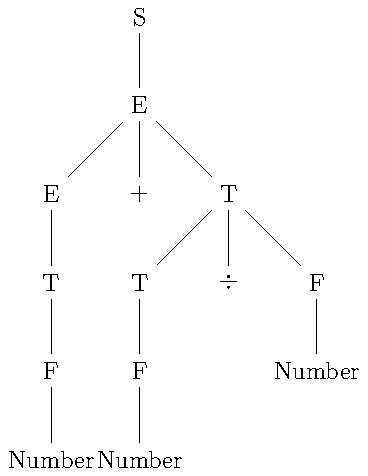
\includegraphics[width=5cm]{img/TP2/2_2a.pdf} }}%
                \qquad
                \subfloat[\centering ]{{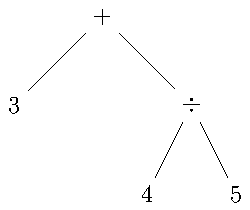
\includegraphics[width=5cm]{img/TP2/2_2b.pdf} }}%
                \caption{AST for 3 + 4/5 and readable AST}
                \label{fig:example}%
            \end{figure}

    \subsubsection{Question2.3}
        \textbf{You will notice that the AST in question 2 does not only reflect the syntactic structure of the
    input but also the precedence of the / operator over the + operator. Add a new operator $<$ to
    the grammar that has lower precedence than the + operator and the / operator and test the
    new grammar on the input $4+7 < 3 + 4/5.$}
    
    \begin{center}
    $ D \rightarrow D < E \ |\  E$ \\
    $ E \rightarrow E + T \ | \  E - T \ | \ T$ \\
    $ T \rightarrow T \cdot F \ | \ T / F \ | \ F$ \\
    $ F \rightarrow (E) \ |\  Number \ | \ Identifier$
\end{center}

    \addimg{img/TP2/2_3b.pdf}{}{}{}

\subsection{Question 3}
    \textbf{Here is a CFG for regular expressions over the alphabet {a, b}. That means the CFG describes how regular expressions look like.}

    \begin{center}
    $ S \rightarrow R $ \\
    $ R \rightarrow R + R \ | \  R R \ | \ R \cdot \ | T $ \\
    $ T \rightarrow (R)  | \ a \ | \ b$ \\
\end{center}

    \textbf{Note that we are using the plus-symbol “+” (e.g., “a+b”) to represent the choice in regular expression $(a|b)$ to avoid confusion with the $|$ used by the CFG itself. Run the NTA of this grammar for the input $a + (b \cdot)$}

    \noindent $(a + (b \cdot), S, \varepsilon)$ \\
$(a + (b \cdot), R, 1)$ Rule 1 to expand S \\
$(a + (b \cdot), R+R, 12)$ Rule 2 to expand S \\
$(a + (b \cdot), T+R, 125)$ Rule 5 to expand R \\
$(a + (b \cdot), a+R, 1257)$ Rule 7 to expand T \\
$( + (b \cdot), +R, 1257)$ Match a\\
$( (b \cdot), R, 1257)$ Match +\\
$( (b \cdot), T, 1257)$ Rule 5 to expand R\\
$( (b \cdot), (R), 125756)$ Rule 6 to expand T\\
$( b \cdot), R), 125756)$ Match (\\
$( b \cdot), R \cdot), 1257564)$ Rule 4 to expand R\\
$( b \cdot), T \cdot), 1257645)$ Rule 5 to expand R\\
$( b \cdot), b \cdot), 125767458)$ Rule 8 to expand R\\
$( \cdot), \cdot), 125767458)$ Match b\\
$( ), ), 125767458)$ Match $\cdot$\\
$( \varepsilon, \varepsilon, 125767458)$ Match )\\


\subsection{Question 4}
    \textbf{Consider the CFG G with the two rules}
    \begin{center}
        $S \rightarrow \ ab \ | \ ac$
    \end{center}
    \textbf{over the terminal symbols $\{a, b, c\}.$}

    \subsubsection{Question 4.1}
        \textbf{Explain why G is not LL(1). Is it LL(2) ?}

        \noindent A grammar is LL(1) if and only if, for all rules 
\begin{center}
    $A \rightarrow \beta | \gamma $ 
    
    $la(A \rightarrow \beta) \cap la(A \rightarrow \gamma) = \varnothing$
\end{center}
with $(\beta \ne \gamma)$  \\

\noindent It is not LL(1) as:
\begin{center}
    $first_{1}(S \rightarrow ab) = first_{1}(S \rightarrow ac) = \{a\}$
\end{center}

\noindent It is LL(2) as:
\begin{center}
    $first_{2}(S \rightarrow ab) = \{ab\} \ne first_{2}(S \rightarrow ac) = \{ac\}$
\end{center}

    \subsubsection{Question 4.2}
        \textbf{Write a CFG that is LL(1) and that generates the same language as G. Hint: the new grammar has two non-terminal symbols.}

        \begin{center}
    $S \rightarrow aR$ \\
    $R \rightarrow b \ | \ c$
\end{center}

    \subsubsection{Question 4.3}
        \textbf{Give a CFG similar to G that is not LL(5)}
        
        \begin{center}
    $S \rightarrow aaaaab \ | \ aaaaac$
\end{center}
